%!TEX root = ../thesis.tex

本研究では，\Fig{fig:proposed}に示すように，高コストなゼロショットセグメンテーション処理と軽量な物体追跡処理を組み合わせる手法を提案する．

\begin{figure}[H]
\centering
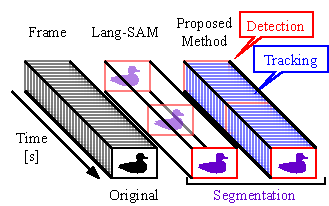
\includegraphics[width=1.0\linewidth]{images/pdf/proposed_method.pdf}
\caption{Overview of the proposed method. (source: \cite{lang_sam_tracker})}
\label{fig:proposed}
\end{figure}

\newpage

この手法は，従来手法のLang-SAMのリアルタイム性を向上させるために Tracking-by-Detection の考え方を応用したものであるが，以下の点が異なる．

第一に，SORTなどが毎フレームの物体検出を前提とするのに対し，本アプローチではゼロショットモデルから成る認識処理を意図的に間引いて実行する．これは，大規模基盤モデルの高い認識性能を維持しつつ，システム全体のスループットを確保するためである．

第二に，物体検出が行われないフレームでは，追跡処理が出力を補間する役割を担う．これにより，高周波な状態更新が求められるモビリティの制御タスクに対応できる可能性がある．

\newpage
